\ctexset{
chapter/name = {\ding{96},},
chapter/number = \arabic{chapter},
section/number = {\arabic{chapter}.\arabic{section}},
}

% \part[东山奈央最萌大赛]{{\Huge\zhongs
% % {\rm\toppanb アニメ最萌トーナメント}\\
% {\minchob 東山奈央}最萌大赛\\闹萌}\\[5em]
% \begin{center}
%  \zihao{4}\rm\kasho {奈央同萌会}
%
%  2017闹萌组委会
% \end{center}}

\newcommand{\By}[1]{
\begin{flushright}
\kai #1
\end{flushright}
}

\setcounter{chapter}{0}

\chapter{预选}

\section{02/22(水) 测试赛~闹曲歌赏}

{\kasho\begin{longtable}{rrl}
\multicolumn{3}{l}{\kai 参赛人数: 131人\quad 合计投出: 1040票} \\
1位 & 48票 & 提督との絆\\
2位 & 42票 & Hello Alone\\
3位 & 40票 & 愛・おぼえていますか\\
4位 & 40票 & 桜色卒業\\
5位 & 33票 & らぶこーる\\
6位 & 27票 & 進め!金剛型四姉妹\\
7位 & 26票 & 想いはRain Rain\\
8位 & 26票 & True Destiny\\
9位 & 25票 & ALL 4 YOU\\
10位 & 23票 & コイノシルシ\\
11位 & 22票 & LOVE KANON\\
11位 & 22票 & エブリデイワールド\\
13位 & 21票 & ハッピークレセント\\
14位 & 19票 & 遠く君へ\\
15位 & 18票 & 恋、ヨロシクお願いします!\\
16位 & 17票 & Live A-Life\\
17位 & 16票 & Angel Breeze\\
18位 & 16票 & Chain the world\\
19位 & 15票 & 瞳からスノー\\
20位 & 15票 & 夏色サプライズ
\end{longtable}}

作为热身赛,前几位的歌曲争夺十分激烈。舰娘和春物ED从中午时刻开始领军,两者交替当首位,知道最后2个小时舰娘才奠定了优势。而三位大部分时间都是沾了超时空要塞delta的热度而异军突起的可曾记得爱。另外需要关注的是并列第三名的樱色卒业,从最开始的第12名一路攀升,最后时刻成功挤进了前三,也是让人捏了一把汗。今天热身结束,明天正赛开始,大家继续为心爱的闹闹角色投票吧。

\By{by 千樱}

本场比赛结果已整理为网易云歌单:~\url{http://music.163.com/#/playlist?id=609555386}

\section{02/23(木) 预选赛1、2组}

{\kai\begin{longtable}{rrl}
\multicolumn{3}{l}{参赛人数: 361人\quad 合计投出: 1730票} \\
\multicolumn{3}{l}{\bfseries Y01 } \\
1位 & 281票 & 由比滨结衣@我的青春恋爱物语果然有问题。 \\
2位 & 238票 & 九条可怜@黄金拼图 \\
3位 & 74票 & 萝特@终末的伊泽塔 \\
4位 & 35票 & 小鸭@生存游戏社! \\
\multicolumn{3}{l}{\xfill{1pt} 此线以上晋级本战 \xfill{1pt}\quad} \\
5位 & 34票 & 露希艾@白猫Project \\
6位 & 33票 & 女仆妹@魔王勇者 \\
7位 & 32票 & 深水阳菜@玻璃之唇 \\
8位 & 28票 & 梅尔薇@巴哈姆特之怒 \\
8位 & 28票 & 宇智波佐助@火影忍者疾风传 \\
10位 & 23票 & 鲁特加尔尼科夫中尉@军人少女 \\
11位 & 19票 & 少女@侵略!乌贼娘 \\
12位 & 17票 & 涉谷光羽@Kiss Bell \\
13位 & 14票 & 村庄的小孩@花之诗女 GOTHICMADE \\
14位 & 13票 & 大渊阳鞠@数码兽世界-next 0rder- \\
15位 & 12票 & 冰见滴@魔术链接 \\
15位 & 12票 & 早乙女葵@落樱散华抄 \\
17位 & 10票 & 诺亚@交响诗篇AO \\
18位 & 9票 & 姿方·泰格@STAR DRIVER 闪亮的塔科特 \\
19位 & 8票 & 博沃洛内@剑与魔法与学园。2G \\
20位 & 6票 & 拉鲁克@太鼓之达人~小龙与不可思议的宝玉 \\
\multicolumn{3}{l}{\bfseries Y02 } \\
1位 & 121票 & 阿波罗@只有神知道的世界 女神篇 \\
2位 & 104票 & 蕾莱·拉·列娜@GATE 奇幻自卫队 \\
3位 & 99票 & 敷波@舰队Collection \\
4位 & 85票 & 茨木童子@Fate/Grand Order \\
\multicolumn{3}{l}{\xfill{1pt} 此线以上晋级本战 \xfill{1pt}\quad} \\
5位 & 80票 & 黑铁珠雫@落第骑士英雄谭 \\
6位 & 56票 & 玛戈特·奈特@境界上的地平线 \\
7位 & 48票 & 凯伊·提亚斯@Regalia 三圣星 \\
8位 & 44票 & 豪德寺佳代@生存游戏社 \\
9位 & 18票 & 维纳斯@幸运逻辑 \\
9位 & 18票 & 寺岛诗织@战姬绝唱Symphogear \\
9位 & 18票 & 学生A@战姬绝唱SYMPHOGEAR \\
12位 & 15票 & 阿涅塔@苍之骑士团 \\
12位 & 15票 & 梅芙@幻兽姬 \\
12位 & 15票 & 白崎莉莉丝@我与一乃的游戏同好会活动日志 \\
12位 & 15票 & 艾莉莎@第101篇百物语 \\
12位 & 15票 & 妖精弓手@哥布林杀手  \\
17位 & 14票 & 达普拉斯M2@机器人少女Z \\
18位 & 13票 & 奥莉薇尔@Cross Ange 天使与龙的轮舞 \\
19位 & 11票 & 日下部雏羽@神影万花镜 时空约定 \\
\end{longtable}}

\B{Y01组}

比赛一开始团子和可怜就抛下了后面的选手交替领先,上午可怜一度确立了领先优势,然而到了中午团子进行了一波爆票,反超后逐渐拉开了与可怜的票差,虽然可怜苦苦追赶,但最后依旧无力回天。最终团子成功获得A组第一并且成为第一天的票王。三位的萝特一直稳扎稳打,全天稳定在三位。反观四位,争夺异常激烈,小鸭、女仆妹、阳菜以及露希艾缠斗了一整天,最后小鸭笑到了最后。

\B{Y02组}

阿波罗的一位无人能撼动,蕾莱在白天的努力下从4位升到了2位,并且确立了与身后的优势。傲娇的敷波表现十分稳定,全天霸占着第三的位置。茨木童子在国服FGO还未登场对她的人气有一定的影响,死忠票集中投完后,一度从2位落到了4位,并且与身后的黑铁珠雫从下午开始一直保持在5票的差距,好在最终有惊无险的晋级了(宣传图角色小组赛出局可不好玩)。

\B{明日看点:}舰娘角色将会大量出场,她们能否创造奇迹,携手晋级呢?

\By{by 琉璃}

\section{02/24(金) 预选赛3、4组}

{\kai\begin{longtable}{rrl}
\multicolumn{3}{l}{参赛人数: 266人\quad 合计投出: 1516票} \\
\multicolumn{3}{l}{\bfseries Y03 } \\
1位 & 188票 & 榛名@舰队Collection \\
2位 & 116票 & 高雄@舰队Collection \\
3位 & 108票 & 莉瑟罗特·沙尔洛克@TRINITY SEVEN 七人魔法使 \\
4位 & 82票 & 克劳蒂雅·恩菲尔德@学战都市Asterisk \\
\multicolumn{3}{l}{\xfill{1pt} 此线以上晋级本战 \xfill{1pt}\quad} \\
5位 & 79票 & 泡芙@Go!公主光之美少女 \\
6位 & 44票 & 圆城寺紫乃@恋爱随意链 \\
7位 & 31票 & 女子A@樱花庄的宠物女孩 \\
8位 & 25票 & 小朋@玉响~more aggressive~ \\
9位 & 20票 & 小早川佐奈@与你一起2 \\
10位 & 16票 & 贞德@新约英雄大戦 \\
11位 & 11票 & 泥泥@青之驱魔师―剧场版― \\
12位 & 10票 & 卡莲@伽利略少女 \\
13位 & 9票 & 越水索菲亚@魔典:私立魔法学园 \\
14位 & 8票 & 伊索德@露蒂的玩具 \\
15位 & 6票 & 莉莉姆·马可拉兹姆@就算要我努力工作 \\
16位 & 4票 & 美联达@武装神姬 BATTLE RONDO \\
17位 & 3票 & 阿拉达·美优@交响诗篇AO \\
17位 & 3票 & 女高音公主@太鼓之达人 小龙与不可思议的宝玉 \\
17位 & 3票 & 椿尤尼@桃色大战 \\
20位 & 1票 & 山口凛子@冬日的誓言 夏日的祭典 武雄的大楠 \\
\multicolumn{3}{l}{\bfseries Y04 } \\
1位 & 139票 & 爱宕@舰队Collection \\
2位 & 124票 & 比叡@舰队Collection \\
3位 & 119票 & 摩耶@舰队Collection \\
4位 & 73票 & 露莉亚@碧蓝幻想 \\
\multicolumn{3}{l}{\xfill{1pt} 此线以上晋级本战 \xfill{1pt}\quad} \\
5位 & 52票 & 小海豹@少年阿瑞GO!GO!小海豹 \\
6位 & 50票 & 蕾克蒂·艾森纳赫@空战魔导士候补生的教官 \\
7位 & 38票 & 川流桃@爱·天地无用! \\
8位 & 22票 & 柏木遥香@初恋之歌 \\
9位 & 18票 & 少女@野良神 \\
10位 & 18票 & 美寻@玉家典当铺 \\
11位 & 17票 & 太田早夜@田中君总是如此慵懒 \\
11位 & 17票 & 米琪·索维斯塔@星之海洋5:忠诚与背叛 \\
13位 & 14票 & 女学生D@我们的肖邦 \\
14位 & 12票 & 春咲日和@公主链接! \\
15位 & 9票 & 荷菈@妖精剑士f \\
16位 & 7票 & 幽子@恶魔奶爸 \\
16位 & 7票 & 亚梅里亚@禁忌的马格纳 \\
18位 & 6票 & 乌苏拉·塔特拉12@棺姬嘉依卡 AVENGING BATTLE \\
19位 & 5票 & 艾芙莉迪·“坂本”·卡布瑞拉@自由战争 \\
20位 & 2票 & 费利西泰@最终流放-银翼之法姆- \\
\end{longtable}}

\B{Y03组}

从比赛开始榛名小天使就牢牢地占据着第一的位置,最终拿到小组第一成为今天的票王。重巡高雄则紧随其后斩下第二,莉瑟罗特也无压力的拿到第三晋级32强。本组的看点在于第四的克劳蒂雅与第五的泡芙(东山狗),尽管一开始会长保持着5票左右的领先,但在泡芙强大的抗压能力下,在下午18点实现反超并且逐渐扩大着优势。本以为会长无力回天,却没想到一股神秘的力量在最后1小时帮助会长最终逆袭,而泡芙则不幸成为第一个小组赛GG的宣传图角色。

\B{Y04组}

本组的焦点在于三位舰娘的内战,本以为比叡会像舰C吧友们说的那样毫无疑问地拿到第一,然而现实是比叡长期处于第三的位置,被棒棒各棒的爱宕和摩耶SAMA牢牢压制,最后结算才超过摩耶拿到第二,爱宕和摩耶分居1、3,不过三位舰娘的票差都不大。四位则由碧蓝幻想的露莉亚夺得,身后的角色并没有对她造成什么威胁,相信动画化后她的人气能更上一层楼。

\B{明日看点:}死亡E05组,几大夺冠热门齐聚小组赛,鹿死谁手,拭目以待!

\By{by 琉璃}

\section{02/25(土) 预选赛5、6组}

{\kai\begin{longtable}{rrl}
\multicolumn{3}{l}{参赛人数: 471人\quad 合计投出: 2167票} \\
\multicolumn{3}{l}{\bfseries Y05 } \\
1位 & 249票 & 桐崎千棘@伪恋 \\
2位 & 246票 & 新子憧@天才麻将少女阿知贺篇 \\
3位 & 192票 & 佐佐木千穗@打工吧!魔王大人 \\
4位 & 191票 & 中川花音@只有神知道的世界 \\
\multicolumn{3}{l}{\xfill{1pt} 此线以上晋级本战 \xfill{1pt}\quad} \\
5位 & 172票 & 鸟海@舰队Collection \\
6位 & 65票 & 猫山铃@犬神同学和猫山同学 \\
7位 & 34票 & 黑崎穗香@向山进发 \\
8位 & 30票 & 犬@微笑光之美少女 \\
9位 & 24票 & 奈奈美@和奈奈美一起学习!English日常会话 \\
10位 & 20票 & 游理/阿斯玛@CLOSERS \\
11位 & 18票 & 卡莉娜@钢之炼金术师 叹息之丘的圣星 \\
12位 & 15票 & 穆西卡@锁链战记 \\
12位 & 15票 & 姑娘@战国少女~桃色异传~ \\
14位 & 11票 & 美沙@小鸡之恋 \\
15位 & 10票 & 巴蒂斯塔@UNDER NIGHT IN-BIRTH \\
15位 & 10票 & 诺巴蒂@X苍炎 失落记忆 \\
17位 & 8票 & 库洛埃·维库尔@CODE GEASS 亡国的阿基德 \\
18位 & 7票 & 梅尔蒂娜·梅尔维斯@穿透幻影的太阳 \\
19位 & 5票 & 丽娃@太鼓之达人 小龙与不可思议的宝玉 \\
\multicolumn{3}{l}{\bfseries Y06 } \\
1位 & 247票 & 金刚@舰队Collection \\
2位 & 116票 & 高坂雪穗@LoveLive! \\
3位 & 98票 & 蕾娜·普劳拉@超时空要塞Δ \\
4位 & 67票 & 室见立华@奋斗吧!系统工程师 \\
4位 & 67票 & 相羽六@魔法战争 \\
\multicolumn{3}{l}{\xfill{1pt} 此线以上晋级本战 \xfill{1pt}\quad} \\
6位 & 41票 & 格琳娜@少女前线 \\
7位 & 35票 & 八月一日静@苍蓝钢铁的琶音 \\
8位 & 33票 & 夕雾@THE UNLIMITED兵部京介 \\
9位 & 31票 & 相乐惠美@临时女友 \\
10位 & 28票 & 中泽工@农林 \\
11位 & 19票 & 露娜露露@要听爸爸的话! \\
12位 & 17票 & 天野望@战斗女子学园 \\
13位 & 9票 & 安娜@真空管少女 \\
14位 & 8票 & 玛丽·安德瓦涅特@世界链接 \\
14位 & 8票 & 迪莫之女@交响诗篇AO \\
16位 & 7票 & 蓓菈@雷姆利亚~Strada Of Chain~\\
17位 & 5票 & 绫@绝灭危愚少女 Amazing Twins \\
18位 & 4票 & 蕾哈涅夫@限界凸骑 \\
19位 & 3票 & 山田佩子@银河机攻队 庄严皇子 \\
20位 & 2票 & 阿古町@乱击!魔法学院 \\
\end{longtable}}

\B{Y05组}

从分组刚出来的时候运营就在大叫“死亡之组”,并为此设置了本战重新分组的规矩。今天一场比赛,果然热闹异常。一开始花音领先,ako紧随其后,千棘则和千穗在同一水平。到了早上,ako开始反超,在中午时分突破百票。下午的比赛突然风向一转,千棘开始逆袭,同时花音越发疲软。晚上千穗开始逐步爆票,直到最后,变成了千棘和ako的一二位之争和千穗和花音的三四位之争。果不其然,两者的差距最后都很小——意料之外登顶的千棘,可能也有情理之中花音的吃四吧。另外舰队的鸟海分到了死亡组,不幸成为首个高票落选的角色。

\B{Y06组}

相对Y05的激烈,Y06的金刚则可以安静地喝红茶,简直是躺赢。本以为能够夺得本日最高票的金刚,却还是大意失荆州以两票之差落于千棘。二位的高坂妹妹保持态势最终破百,三位的蕾娜也很稳定。只有4、5、6位的晋级之争,伴随着隔壁的如火如荼,也是异常激烈。最开始室见立华领先一两票,然后相羽六和格琳娜纷纷在白天追上,午后时分一度超过。下午,随着立华的一波爆票,格琳娜变得疲软,立华和相羽六开始维持平票态势。票数缓慢增加,直到最后稍有波动,达成平票晋级的结果。

今天参赛人数达到471人,创下了新高。

\B{明日看点:}Y07组变数较多,Y08看似晋级稳定却也暗藏波澜,欢迎大家继续投票。

\By{by 自由}

\section{02/26(日) 预选赛7、8组}

{\kai\begin{longtable}{rrl}
\multicolumn{3}{l}{参赛人数: 126人\quad 合计投出: 727票} \\
\multicolumn{3}{l}{\bfseries Y07 } \\
1位 & 63票 & 伊万莉玛丽亚@这个美术部大有问题 \\
2位 & 61票 & 绫波@舰队Collection \\
3位 & 56票 & 川岛瑞树@偶像大师灰姑娘女孩 \\
4位 & 43票 & 潮田渚@暗杀教室OAD \\
\multicolumn{3}{l}{\xfill{1pt} 此线以上晋级本战 \xfill{1pt}\quad} \\
5位 & 35票 & 夏川真那@我女友与青梅竹马的惨烈修罗场 \\
6位 & 26票 & 迦具夜@机巧少女不会受伤Facing "Burnt Red" \\
7位 & 22票 & 仓田亚美@长骑美眉 \\
8位 & 18票 & 江口结瞳@噬血狂袭 OVA II \\
9位 & 16票 & 西尔维娅·斑鸠·御折木@Cross Ange 天使与龙的轮舞 \\
10位 & 11票 & 桃子@樱花庄的宠物女孩 \\
11位 & 8票 & 过路人\#6@恶魔阿萨谢尔在召唤你 \\
12位 & 7票 & 狭间菜月@「一起睡觉吧」广播剧 \\
13位 & 5票 & 王者之剑@青之驱魔师 \\
14位 & 3票 & 维拉@AKB0048 \\
15位 & 1票 & 濑波光@武装中学生 \\
15位 & 1票 & 君岛文香@欺凌 \\
15位 & 1票 & 公主@星霜的亚马逊人 \\
15位 & 1票 & Sierra Los@GE 王者之剑 \\
15位 & 1票 & 伊藤初芽@胖嘟嘟游泳社 \\
20位 & 0票 & 莉珂莉丝·罗薇娜@梦幻模拟战:转生 \\
\multicolumn{3}{l}{\bfseries Y08 } \\
1位 & 67票 & 雾岛@舰队Collection \\
2位 & 58票 & 白雪@魔法少女育成计划 \\
3位 & 55票 & 汤音@异国迷宫的十字路口 \\
4位 & 48票 & 铃乃木凛@爆音少女!! \\
\multicolumn{3}{l}{\xfill{1pt} 此线以上晋级本战 \xfill{1pt}\quad} \\
5位 & 46票 & 伞木希美@吹响!上低音号2 \\
6位 & 15票 & 卑弥呼@愚者信长 \\
7位 & 12票 & 高见泽亚里沙@~告白实行委员会~ \\
8位 & 10票 & 皮克西@魔法科高中的劣等生 \\
8位 & 10票 & 米海鲁@誓血龙骑士3 \\
10位 & 7票 & 女高中生\#5@恶魔阿萨谢尔在召唤你 \\
11位 & 4票 & 菲斯堤妮亚·谬斯@超级机器人大战OG THE MOON DWELLERS \\
12位 & 3票 & 光武伊莉娜@偶像事变 \\
12位 & 3票 & 犬神@妖怪百姬 \\
12位 & 3票 & 小孩@闪光的夜袭 \\
15位 & 2票 & 相良美宇@记录之恋 蓝色海洋/金色沙滩 \\
15位 & 2票 & 库洛诺斯·库罗尼卡@桃色大战 \\
17位 & 1票 & 美芙·麦卡佛瑞@交响诗篇AO \\
17位 & 1票 & 星灵·贝尔@星界神话 \\
17位 & 1票 & 丸山幸@1518 \\
20位 & 0票 & 艾玛·提格里斯@JK吸血鬼~命运的祭典~ \\
\end{longtable}}

\B{Y07组}

相比昨天的激烈竞争,今天出场的角色都不是特别强势,比赛也冷淡了许多。Y07组一开始伊万莉就守住了Top直到比赛结束。绫波以不差很多的票数,一直在第二。三位的灰姑娘川岛瑞树,作为东山少数“大姐姐”声线的偶像角色,并不是特别强力。4位本来是夏川真那一直把手,然而下午从贴吧来的一波爆票,直接把潮田渚推上了晋级——成为唯一一个晋级本战的男孩子。另外的长骑美眉的仓田亚美和噬血狂袭江口结瞳意外落榜,还有天使龙的小公主,确实不够有力啊。

\B{Y08组}

雾岛分到了一个弱组,和昨天的金刚一样躺赢,票数却差了好多。白雪顺利保住二位。闹闹的早期角色汤音,在度过了略有危险的一天后,不负众望晋级。爆音少女的铃木爱好者铃乃木凛和上低音号的伞木希美前辈从下午开始竞争,凛最后以两票微弱优势进入本战。其他角色则票数过少,甚至出现了久违的0票。

\B{明日看点:}本战分组将直接决定16强和八强名额,欢迎继续关注。

\By{by 自由}

\section{02/27(月) 表演赛I}

{\kai\begin{tabular}{rrl}
\multicolumn{3}{l}{参赛人数: 112人\quad 合计投出: 375票} \\
\multicolumn{3}{l}{\bfseries 四大神兽 } \\
1位 & 41票 & 泡芙@Go!公主光之美少女 \\
2位 & 23票 & 小鸭@生存游戏社! \\
3位 & 19票 & 小海豹@少年阿瑞GO!GO!小海豹 \\
4位 & 7票 & 米海鲁@誓血龙骑士3 \\
\multicolumn{3}{l}{\bfseries 金刚四傻 } \\
1位 & 60票 & 金刚@舰队Collection \\
2位 & 25票 & 榛名@舰队Collection \\
3位 & 7票 & 比叡@舰队Collection \\
4位 & 6票 & 雾岛@舰队Collection \\
\end{tabular}\begin{tabular}{rrl}
\multicolumn{3}{l}{} \\
\multicolumn{3}{l}{\bfseries 四大子供 } \\
1位 & 53票 & 光之美少女@系列 \\
2位 & 17票 & 偶像活动@系列 \\
3位 & 15票 & 美妙旋律@系列 \\
4位 & 5票 & 宝石宠物@系列 \\
\multicolumn{3}{l}{\bfseries 四大业界 } \\
1位 & 52票 & 京都动画@知名动画制作公司 \\
2位 & 21票 & 山本宽@知名动画导演 \\
3位 & 20票 & 虚渊玄@知名动画编剧 \\
4位 & 4票 & 秋元康@知名偶像制作人 \\
\end{tabular}}

\begin{center}
  \quad
\end{center}

表演赛第一场的同时进行了本战分组,具体分组见下页表格。

\newpage
\markboth{本战晋级表}{}
\CTEXnoindent
{
\begin{tabular}{|l|p{20em}|c|c|c|c|c|}
\hline
\multicolumn{2}{|c|}{\hei{A 组}} & \multicolumn{2}{c|}{\hei{一回战}} & \multicolumn{2}{c|}{\hei{二回战}} \\ \hline
\B{A-1} & \B{中川花音@只有神知道的世界} & \B{151} & \Cell{2}{2月28日\\\B{中川花音}} & \multirow{2}{*}{\B{155}} & \Cell{5}{3月4日\\\B{中川花音}}\\ \cline{1-3}
A-2 & 蕾娜·普劳拉@超时空要塞Δ & 57 & & & \\ \cline{1-5}
A-3 & 蕾莱·拉·列娜@$\!$GATE 奇幻自卫队 & 54 & \Cell{3}{3月2日\\\B{绫波}} & \multirow{3}{*}{70} & \\ \cline{1-3}
\B{A-4} & \B{绫波@舰队Collection} & \B{57} & & & \\ \cline{1-3}
A-5 & 潮田渚@暗杀教室OAD & 18 & & & \\ \hline
\hline
\multicolumn{2}{|c|}{\hei{B 组}} & \multicolumn{2}{c|}{\hei{一回战}} & \multicolumn{2}{c|}{\hei{二回战}} \\ \hline
  {B-1} & 高坂雪穗@$\!$LoveLive! & 94 & \Cell{2}{2月28日\\\B{雾岛}} & \multirow{2}{*}{{134}} & \Cell{4}{3月4日\\\B{桐崎千棘}}\\ \cline{1-3}
\B{B-2} & \B{雾岛@舰队Collection} & \B{109} & & & \\ \cline{1-5}
  {B-3} & 阿波罗@只有神知道的世界 女神篇 & 35 & \Cell{2}{3月2日\\\B{桐崎千棘}} & \multirow{2}{*}{\B{141}} & \\ \cline{1-3}
\B{B-4} & \B{桐崎千棘@伪恋} & \B{108} & & & \\ \hline
\end{tabular}
}
\CTEXindent


\chapter{本战}

\section{02/28(火) 本战1回战~ABCD上}

{\kai\begin{longtable}{rrl}
\multicolumn{3}{l}{参赛人数: 232人\quad 合计投出: 845票} \\
\multicolumn{3}{l}{\bfseries A-1 A-2 } \\
1位 & 151票 & 中川花音@只有神知道的世界 \\
2位 & 57票 & 蕾娜·普劳拉@超时空要塞Δ \\
\multicolumn{3}{l}{\bfseries B-1 B-2 } \\
1位 & 109票 & 雾岛@舰队Collection \\
2位 & 93票 & 高坂雪穗@LoveLive! \\
\multicolumn{3}{l}{\bfseries C-1 C-2 } \\
1位 & 171票 & 由比滨结衣@我的青春恋爱物语果然有问题。 \\
2位 & 44票 & 伊万莉玛丽亚@这个美术部大有问题 \\
\multicolumn{3}{l}{\bfseries D-1 D-2 } \\
1位 & 139票 & 金刚@舰队Collection \\
2位 & 81票 & 佐佐木千穗@打工吧!魔王大人 \\
\end{longtable}}

\B{A组}

终于进入1v1的本战了,第一场就是闹厨最爱的花音。旧时代偶像中川花音vs新时代偶像蕾娜普劳拉,新旧偶像的对决本以为会有不小冲突——这场看来女武神的单人战斗力还是不足啊,尤其是无口属性的蕾娜。花音从一开始就占据领先地位,毫无悬念地晋级二回战。

\B{B组}

这是今天最为难以预料的一组,舰娘的几乎最不人气角色大战果皇妹妹。开场雾岛领先微弱,高坂雪穗则在上午一度反超。中午之后,雾岛重新占据领先地位,之后票差一直维持着16票左右,拉拉⑨人外角色止步一回战。

\B{C组}

乍一看两人长得这么像,会不会有姬情啊?团子是预选赛票王,这场也展示了不俗的皮票力。同是团子头的伊万莉则没那么强势,开场便倒在团子石榴裙下,一天比赛之中票差也越拉越大,有一个蛤蟆桑成功晋级。

\B{D组}

作为预选票数前8的两名角色分到了同一组,非常瞩目。然而,金刚的人气实在是太高——作为舰队的主力,显然比几年前的小千有力得多。即便是小千换上了颜艺甚至是颜艺的动图,也动摇不了大傻的绝对地位。请大家记住佐佐木千穂——的颜艺!

\B{明日看点:}绝对王者出场对阵偶像大师,试问鹿死谁手?

\By{by 自由}

\section{03/01(水) 本战1回战~EFGH上}

{\kai\begin{longtable}{rrl}
\multicolumn{3}{l}{参赛人数: 159人\quad 合计投出: 556票} \\
\multicolumn{3}{l}{\bfseries E-1 E-2 } \\
1位 & 114票 & 新子憧@天才麻将少女阿知贺篇 \\
2位 & 38票 & 川岛瑞树@偶像大师灰姑娘女孩 \\
\multicolumn{3}{l}{\bfseries F-1 F-2 } \\
1位 & 108票 & 九条可怜@黄金拼图 \\
2位 & 40票 & 摩耶@舰队Collection \\
\multicolumn{3}{l}{\bfseries G-1 G-2 } \\
1位 & 83票 & 敷波@舰队Collection \\
2位 & 47票 & 小鸭@生存游戏社! \\
\multicolumn{3}{l}{\bfseries H-1 H-2 } \\
1位 & 74票 & 铃乃木凛@爆音少女!! \\
2位 & 52票 & 露莉亚@碧蓝幻想 \\
\end{longtable}}

\B{E组}

本战进入第二天,绝对王者面对偶像大师,毫无压力的轻松拿下,大姐姐瑞树也是早早就放弃了抵抗,全天的票差也是越拉越大。最终ako拿到今天全场的最高票强势晋级二回战,我们期待她接下来的表现。

\B{F组}

与舰C的角色金刚同样是归国子女的可怜,面对摩耶SAMA也是早早就确立了优势,同时也展现了不俗的票力,终场拿到仅次于ako的票数desu

\B{G组}

敷波和小鸭这组还是比较有看点的,驱逐舰和神兽开场咬得还是比较紧的,随着白天投票人数的增加,敷波逐渐确立起了优势,最终有惊无险地淘汰了预选赛的黑马小鸭

\B{H组}

骑车少女对抗迷之美少女,开场在碧蓝幻想死忠的支持下,露莉亚与凛的票数相差无几。但是到了白天逐渐显露出了动画化作品的影响力,凛也在下午拉开到十几票的差距并持续稳定到结束,今年4月才动画化的碧蓝也使得露莉亚止步32强

\B{明日看点:}A组下半区三人混战,究竟谁能脱颖而出?B组下半区花音小号阿波罗挑战夺冠热门千棘,千棘能否展现冠军实力值得期待。CD两组各有一位魔法少女出战,她们是否可以同时出现?

\By{by 琉璃}

\section{03/02(木) 本战1回战~ABCD下}

{\kai\begin{longtable}{rrl}
\multicolumn{3}{l}{参赛人数: 152人\quad 合计投出: 508票} \\
\multicolumn{3}{l}{\bfseries A-4 A-5 A-6 } \\
1位 & 57票 & 绫波@舰队Collection \\
2位 & 54票 & 蕾莱·拉·列娜@GATE 奇幻自卫队 \\
3位 & 18票 & 潮田渚@暗杀教室OAD \\
\multicolumn{3}{l}{\bfseries B-3 B-4 } \\
1位 & 108票 & 桐崎千棘@伪恋 \\
2位 & 35票 & 阿波罗@只有神知道的世界 女神篇 \\
\multicolumn{3}{l}{\bfseries C-3 C-4 } \\
1位 & 64票 & 白雪@魔法少女育成计划 \\
2位 & 52票 & 萝特@终末的伊泽塔 \\
\multicolumn{3}{l}{\bfseries D-3 D-4 } \\
1位 & 70票 & 高雄@舰队Collection \\
2位 & 50票 & 相羽六@魔法战争 \\
\end{longtable}}

\B{A组}

下半区的战斗今天打响,由于预选赛平票晋级的关系,首次出现了三人一组的情况,然而渚貌似早早就放弃了比赛,毕竟这个角色还是本篇的人气高。驱逐舰绫波和魔导少女蕾莱从开场到最后始终难分胜负,从早上绫波的微微领先,到下午蕾莱的爆票反超,以及终场的绫波再次反超,57:54,驱逐舰笑到了最后。

\B{B组}

夺冠热门千棘并没有给花音小号阿波罗爆冷的机会,一开始便牢牢掌握优势,并逐渐拉开票差,最终以108的今日最高票毫无悬念的晋级。

\B{C组}

魔法少女与女仆的战斗也是相爱相杀了一整天,白天始终是萝特的领先,但是票差始终保持在个位数,这也给了白雪晚上反超的机会,终于最后在一波爆票后,白雪逆转12票晋级。

\B{D组}

相比上一组的魔法少女,这组的相羽六全天被高雄大姐姐压制,尽管票差不算很大,但也始终没有足够的底气缩小差距,可能也是因为魔法战争动画本身的原因,最终舰C又抢夺了一个16强的席位。

\B{明日看点:}舰C势力再出发,分布三组的她们是否能携手晋级?

\By{by 琉璃}

\newpage
\section{03/03(金) 本战1回战~EFGH下}

{\kai\begin{longtable}{rrl}
\multicolumn{3}{l}{参赛人数: 129人\quad 合计投出: 458票} \\
\multicolumn{3}{l}{\bfseries E-3 E-4 } \\
1位 & 62票 & 比叡@舰队Collection \\
1位 & 62票 & 汤音@异国迷宫的十字路口 \\
\multicolumn{3}{l}{\bfseries F-3 F-4 } \\
1位 & 89票 & 爱宕@舰队Collection \\
2位 & 26票 & 茨木童子@Fate/Grand Order \\
\multicolumn{3}{l}{\bfseries G-3 G-4 } \\
1位 & 84票 & 榛名@舰队Collection \\
2位 & 34票 & 莉瑟罗特·沙尔洛克@TRINITY SEVEN 七人魔法使 \\
\multicolumn{3}{l}{\bfseries H-3 H-4 } \\
1位 & 53票 & 室见立华@奋斗吧!系统工程师 \\
2位 & 48票 & 克劳蒂雅·恩菲尔德@学战都市Asterisk \\
\end{longtable}}

\B{E组}

今天的E组是闹萌本战开赛以来首次出现同票的一组,也恭喜汤音比叡一起携手进入二回战。比赛开始时,汤音占据较为明显的优势,可见小萝莉真爱党们都比较积极,到了下午比叡的票数开始有了明显增长,但是两者之间还是有着微弱的差距,但是这点差距在舰C势力的眼中不值一提,到了晚上8点-9点这段时间票数逐渐追平,最终定格于62票与汤音同票。再次感叹下舰C势力的强大战斗力。

\B{F组}

从开赛开始基本没有悬念,棒棒个棒一路领先,以几乎碾压的姿态完胜茨木童子,果然应证了一句老话--乳不巨何以聚人心啊(大雾)。恭喜爱宕最终以大比分优势成功晋级。

\B{G组}

G组比赛也是没有任何悬念的就结束了,魔法师还是斗不赢小天使啊,这也再次证明了舰C势力的强大,作为闹闹的代表角色之一,也希望小天使可以在接下来的二回战中取得更好的成绩。

\B{H组}

本组的比赛算是一波三折了,程序员和学姐一直都在激战之中,票数几乎一直处于持平的趋势,虽然有动画热度的加成,但是对上了程序员的学姐也依然没有特别大的优势,可见喜欢程序员妹子的萌豚们也不容小觑呢(滑稽)。总之,恭喜立华以微弱的优势取得本场胜利,也希望喜欢程序员妹子的人越来越多。

\B{明日看点:}舰C势力能否继续独领风骚?人气角色战力究竟几何?尽情期待明日之战!

\By{by 游离}

\newpage
\section{03/04(土) 本战2回战~上半区}

{\kai\begin{longtable}{rrl}
\multicolumn{3}{l}{参赛人数: 296人\quad 合计投出: 957票} \\
\multicolumn{3}{l}{\bfseries 本战A } \\
1位 & 155票 & 中川花音@只有神知道的世界 \\
2位 & 70票 & 绫波@舰队Collection \\
\multicolumn{3}{l}{\bfseries 本战B } \\
1位 & 141票 & 桐崎千棘@伪恋 \\
2位 & 134票 & 雾岛@舰队Collection \\
\multicolumn{3}{l}{\bfseries 本战C } \\
1位 & 204票 & 由比滨结衣@我的青春恋爱物语果然有问题。 \\
2位 & 35票 & 白雪@魔法少女育成计划 \\
\multicolumn{3}{l}{\bfseries 本战D } \\
1位 & 157票 & 金刚@舰队Collection \\
2位 & 61票 & 高雄@舰队Collection \\
\end{longtable}}

\B{A组}

花音今天状态良好,比赛开始就一路领先于凌波,最终以155票的成绩取得本场比赛胜利。首先恭喜咱们的偶像一路披荆斩棘,获得了8强赛的入场券,也希望花音酱能在8强中持续发力,取得更好的成绩!{\mincho LOVEカノンの光、あなたの心を照らすだよ!}

\B{B组}

本场比赛乃是今天最为持久和激烈的拉锯战,赛程开始时,千棘优势明显,谁知雾岛中程发力,一举反超千棘,大大振奋了舰C势力的军心,可是千棘真爱党们哪里能示弱,在中后段的比赛里奋起直追,直至追平比分。这场精彩的攻防战看得人直呼过瘾,最终千棘以微弱的优势战胜了舰C势力大咖之一的雾岛,成功晋级8强!

\B{C组}

团子的强大远超想象,以近乎碾压的姿态战胜白雪,强势闯进8强,白雪也不要再哭啦\verb=~~(>_<)~~=摸头,毕竟对手可是闹萌的BOSS之一呢。在这里祝贺结衣,期待你在8强赛的表现!

\B{D组}

本组比赛虽说是舰C势力的内战,但是金刚作为领袖人物,依然保持着舰C大姐头的风采,闹萌中舰C势力虽然庞大,但也避免不了赛程中损兵折将,高雄最终惜败。恭喜金刚挺入8强,相信能集合更多优势资源,鏖战各大萌主,让我们拭目以待吧!

\B{明日看点:}八强名额还剩四席,明日又会花落谁家?会是种子选手成功出线,又或黑马之王顽强逆袭?尽情期待明日之战!

\By{by 游离}

\newpage
\section{03/05(日) 本战2回战~下半区}

{\kai\begin{longtable}{rrl}
\multicolumn{3}{l}{参赛人数: 363人\quad 合计投出: 804票} \\
\multicolumn{3}{l}{\bfseries 本战E } \\
1位 & 113票 & 新子憧@天才麻将少女阿知贺篇 \\
2位 & 73票 & 比叡@舰队Collection \\
3位 & 41票 & 汤音@异国迷宫的十字路口 \\
\multicolumn{3}{l}{\bfseries 本战F } \\
1位 & 130票 & 九条可怜@黄金拼图 \\
2位 & 95票 & 爱宕@舰队Collection \\
\multicolumn{3}{l}{\bfseries 本战G } \\
1位 & 157票 & 榛名@舰队Collection \\
2位 & 34票 & 敷波@舰队Collection \\
\multicolumn{3}{l}{\bfseries 本战H } \\
1位 & 84票 & 铃乃木凛@爆音少女!! \\
2位 & 77票 & 室见立华@奋斗吧!系统工程师 \\
\end{longtable}}

\B{E组}

一回战的时候汤音与比叡战了一个55开,于是二回战又出现了三人一组的情况,不过面对绝对王者,她们似乎没有太多的机会,除了一开始的散票支撑之外,ako全天都处于遥遥领先的地位,轻松晋级,我们期待在8强赛中她能有更精彩的表现。

\B{F组}

一回战的时候可怜对上的是重巡,二回战同样对上的也是重巡。一心想为舰C同胞复仇的爱宕全天的机会并不多,倒是晚上的一波爆票略微考验了一下可怜,最终可怜以130:95的成绩晋级。8强赛中很希望能看到可怜和金刚的对决,不知道能否实现呢?

\B{G组}

这又是一场舰C的内战,相比于傲娇的驱逐舰敷波,大家选择了战斗力更强的战舰榛名,小天使也是毫无悬念的晋级8强。之前的表演赛中小天使不敌大姐金刚,8强战中会不会让她们有再次战斗的机会呢?

\B{H组}

谁都没想到铃乃木凛与室见立华能走到这一步,然而分组也是实力之一。今天她们也是打的难解难分,从开局的平票到白天的互有领先,不到最后一刻无法决出胜负。最终骑摩托妹子艰难战胜程序员妹子,拿到了最后一个8强席位。

\B{明日看点:}8强分组值得期待,表演赛内容也很丰富,欢迎大家多多参与!

\By{by 琉璃}

\newpage
\section{03/06(月) 表演赛II}

{\kai\begin{longtable}{rrl}
\multicolumn{3}{l}{参赛人数: 106人\quad 合计投出: 295票} \\
\multicolumn{3}{l}{\bfseries 闹的CP } \\
1位 & 62票 & 佐仓绫音@I'm Enterprise \\
2位 & 30票 & 早见沙织@I'm Enterprise \\
3位 & 6票 & 内山夕实@ARTSVISION \\
4位 & 5票 & 山崎遥@ARTSVISION \\
\multicolumn{3}{l}{\bfseries 业界氪金王 } \\
1位 & 27票 & 悠木碧@Pro·Fit \\
2位 & 26票 & 三泽纱千香@Space Craft Entertainment \\
3位 & 23票 & 竹达彩奈@Assemble Heart \\
4位 & 20票 & 岛崎信长@青二Production \\
\multicolumn{3}{l}{\bfseries 热门手游 } \\
1位 & 31票 & 偶像大师灰姑娘女孩星光舞台@BANDAI NAMCO Entertainment \\
2位 & 31票 & 命运-冠位指定@DELiGHTWorks \\
3位 & 19票 & LoveLive!@Klabgames \\
4位 & 15票 & 阴阳师@网易移动游戏 \\
\end{longtable}}

表演赛第二场的同时进行了决赛圈分组,8人随机分为东南西北4组,进行交叉对战。

\chapter{决赛}

\begin{center}
\renewcommand\baselinestretch{2}\selectfont
\begin{tabular}{|c|c|l|c|}
\hline
\Cell{2}{3月11日\\[-1em]\kai 萌王战} & ① & \B{由比滨结衣@我的青春恋爱物语果然有问题。} & \B{346} \\\cline{2-4}
 & ② & 桐崎千棘@伪恋 & 274\\\hline
 \Cell{2}{3月10日\\[-1em]\kai 三位战} & ③ & \B{中川花音@只有神知道的世界} & \B{83} \\\cline{2-4}
  & ④ & 新子憧@天才麻将少女阿知贺篇 & 63\\\hline
\end{tabular}\renewcommand\baselinestretch{1.4}\selectfont
\end{center}
\quad\\
\begin{center}
\renewcommand\baselinestretch{1.5}\selectfont
\begin{tabular}{|c|l|c|c|c|c|}
\hline
\multicolumn{3}{|c|}{\hei{八强}} & \multicolumn{3}{c|}{\hei{四强}} \\ \hline
\multirow{2}{*}{\huge\AppleSymbols 🀀} & \B{新子憧@天才麻将少女阿知贺篇} & \B{93} & \Cell{2}{3月7日\\[-.4em]{新子憧}} & \multirow{2}{*}{175} & \Cell{4}{3月9日\\\B{由比滨结衣}}\\ \cline{2-3}
 & 金刚@舰队Collection & 80 & & & \\ \cline{1-5}
 \multirow{2}{*}{\huge\AppleSymbols 🀂} & 榛名@舰队Collection & 157 & \Cell{2}{3月8日\\[-.4em]\B{由比滨结衣}} & \multirow{2}{*}{\B{261}} & \\ \cline{2-3}
  & \B{由比滨结衣@我的青春恋爱物语果然有问题。} & \B{390} & & & \\ \cline{1-6}
\multirow{2}{*}{\huge\AppleSymbols 🀁} & 铃乃木凛@爆音少女!! & 45 & \Cell{2}{3月7日\\[-.4em]{中川花音}} & \multirow{2}{*}{200} & \Cell{4}{3月9日\\{桐崎千棘}}\\ \cline{2-3}
 & \B{中川花音@只有神知道的世界} & \B{114} & & & \\ \cline{1-5}
 \multirow{2}{*}{\huge\AppleSymbols 🀃} & \B{桐崎千棘@伪恋} & \B{296} & \Cell{2}{3月8日\\[-.4em]\B{桐崎千棘}} & \multirow{2}{*}{\B{239}} & \\ \cline{2-3}
  & 九条可怜@黄金拼图 & 274 & & & \\ \cline{1-6}
\end{tabular}\renewcommand\baselinestretch{1.4}\selectfont
\end{center}

\newpage
\section{03/07(火) 八进四~东南组}

{\kai\begin{longtable}{rrl}
\multicolumn{3}{l}{参赛人数: 181人\quad 合计投出: 332票} \\
\multicolumn{3}{l}{\bfseries 東 } \\
1位 & 93票 & 新子憧@天才麻将少女阿知贺篇 \\
2位 & 80票 & 金刚@舰队Collection \\
\multicolumn{3}{l}{\bfseries 南 } \\
1位 & 114票 & 中川花音@只有神知道的世界 \\
2位 & 45票 & 铃乃木凛@爆音少女!! \\
\end{longtable}}

\B{东组}

进入8强以后果然战况激烈,金刚与ako全天互有领先,票差始终在个位数,短暂的交锋后,金刚与下午开始保持领先,然而绝对王者没有放弃,始终紧咬票数,在最后半小时只落后3票,没想到的是在最后的最后还进行了一波爆票,而金刚领先了那么长时间居然在最后疲软了,最终ako成功完成海底反杀,晋级4强。

\B{南组}

相比于东组的激烈对决,花音则对上了本届的黑马铃乃木凛,结果却是花音的一边倒胜利。黑马终究是黑马,在8强这样的环境下,过硬的实力才是晋级的资本,也恭喜花音拿到一个四强的席位。

\By{by 琉璃}

\section{03/08(水) 八进四~西北组}

{\kai\begin{longtable}{rrl}
\multicolumn{3}{l}{参赛人数: 1629人\quad 合计投出: 1117票} \\
\multicolumn{3}{l}{\bfseries 西 } \\
1位 & 390票 & 由比滨结衣@我的青春恋爱物语果然有问题。 \\
2位 & 157票 & 榛名@舰队Collection \\
\multicolumn{3}{l}{\bfseries 北 } \\
1位 & 296票 & 桐崎千棘@伪恋 \\
2位 & 274票 & 九条可怜@黄金拼图 \\
\end{longtable}}

\B{西组}

上午团子就和榛名拉开了票差,不过下午开始榛名党开始反(shua)击(piao),尽管如此,舰娘中最适合当人妻的榛名的票数始终也只是接近而没有反超,可见团子强大的人气。最后在运营砍掉多重之后团子大比分的领先榛名晋级四强。

\B{北组}

北组今天真是火药味十足,千棘和可怜两个归国子女打的是不可开交。从上午开始就交替领先。下午开始则有几个厨开始疯狂刷票。开始运营还实时砍,后来决定砍票的结果最后再放出来以增加娱乐性。之后伪票数一度破千。最后结果出来,千棘以22票的微弱优势险胜可怜。闹闹唯一的胜者角色也成功晋级四强。

\B{明日看点:}人气王团子大战世界第一Ako,傲娇千棘对战情怀花音

\By{by 千樱}

\section{03/09(木) 半决赛}

{\kai\begin{longtable}{rrl}
\multicolumn{3}{l}{参赛人数: 477人\quad 合计投出: 875票} \\
\multicolumn{3}{l}{\bfseries 東西 } \\
1位 & 261票 & 由比滨结衣@我的青春恋爱物语果然有问题。 \\
2位 & 175票 & 新子憧@天才麻将少女阿知贺篇 \\
\multicolumn{3}{l}{\bfseries 南北 } \\
1位 & 239票 & 桐崎千棘@伪恋 \\
2位 & 200票 & 中川花音@只有神知道的世界 \\
\end{longtable}}

\B{东西组}

从团子一路晋级的比赛来看,只要是她出场的比赛总是能拿到全天的最高票,尽管半决赛的对手是绝对王者ako,团子依旧展现出她强大的战斗力。全天一直处于领先的团子让ako看到了一个梗无法通吃所有比赛,最终团子获得了决赛的门票,而ako将于明天争夺第三位。

\B{南北组}

作为闹闹出演动画里唯一取得胜利的角色,傲娇千棘对上了闹闹的起点情怀花音。这是一场让人纠结的比赛,花音一度与千棘打成了55开,但是毕竟时代前进了,千棘作为新时代的女主自然拥有更多的人气。虽然花音始终没有放弃,但最后也无力回天,明天将与ako进行三位争夺战,而千棘则是在后天与团子进行最终的萌王战。

\B{明日看点:}绝对王者VS情怀偶像

\By{by 琉璃}

\section{03/10(金) 三位战}

{\kai\begin{longtable}{rrl}
\multicolumn{3}{l}{参赛人数: 147人\quad 合计投出: 146票} \\
\multicolumn{3}{l}{\bfseries 三四位 } \\
1位 & 83票 & 中川花音@只有神知道的世界 \\
2位 & 63票 & 新子憧@天才麻将少女阿知贺篇 \\
\end{longtable}}

\B{三位战}

闹萌逐渐接近尾声,三位战似乎在为明天的决赛蓄力,今天的总票数算不上太多,但这场比赛也十分精彩。开局阶段花音与ako齐头并进,互有领先,随着比赛的进行,情怀党主导了比赛的走向,花音从下午开始一直领先并保持到了终场,麻将王者最终只能屈居第四,我们也祝贺花音拿下三位。

\B{明日看点:}闹闹生日当天的决赛,人气天王大战唯一胜者,萌王花落谁家?

\By{by 琉璃}

\section{03/11(土) 萌王战}

{\kai\begin{longtable}{rrl}
\multicolumn{3}{l}{参赛人数: 2474人\quad 合计投出: 622票} \\
\multicolumn{3}{l}{\bfseries 决赛 } \\
1位 & 346票 & 由比滨结衣@我的青春恋爱物语果然有问题。 \\
2位 & 276票 & 桐崎千棘@伪恋 \\
\end{longtable}}

\B{萌王战}

在迎来东山奈央25岁生日之际,2017届闹萌也敲响了萌王战的战鼓。不愧是东山双雄,开场便激烈地开展了争斗。团子开场领先一波,随后被千棘追上。团子在半夜,始终保持着对千棘的微弱优势,直到白天。中午,千棘开始爆票。于是,千棘成功反超并逐渐远超团子。团子党午后发现事态不对,迅速组织了一波开始爆票。显然,两家开始了强大的对轰。这一轰不要紧,加上晚上的海啸,两家各轰出了上千票!比赛结束,集计结果,千棘1439:1033团子。

这票数看起来很漂亮,但是用心的运营从后台来看,是明显的厨团出票。除了非常简单的多重之外,出现了大量异常各式型号手机的投票。很显然,这些票对正常比赛产生了相当大的影响。运营组集体商讨之后,标记了这些无效票。最终审议集计结果为,团子346:276千棘。2017闹萌在一片喧闹之中落幕,由比滨结衣当选首届闹萌萌王。

\By{by 自由}

\begin{center}
{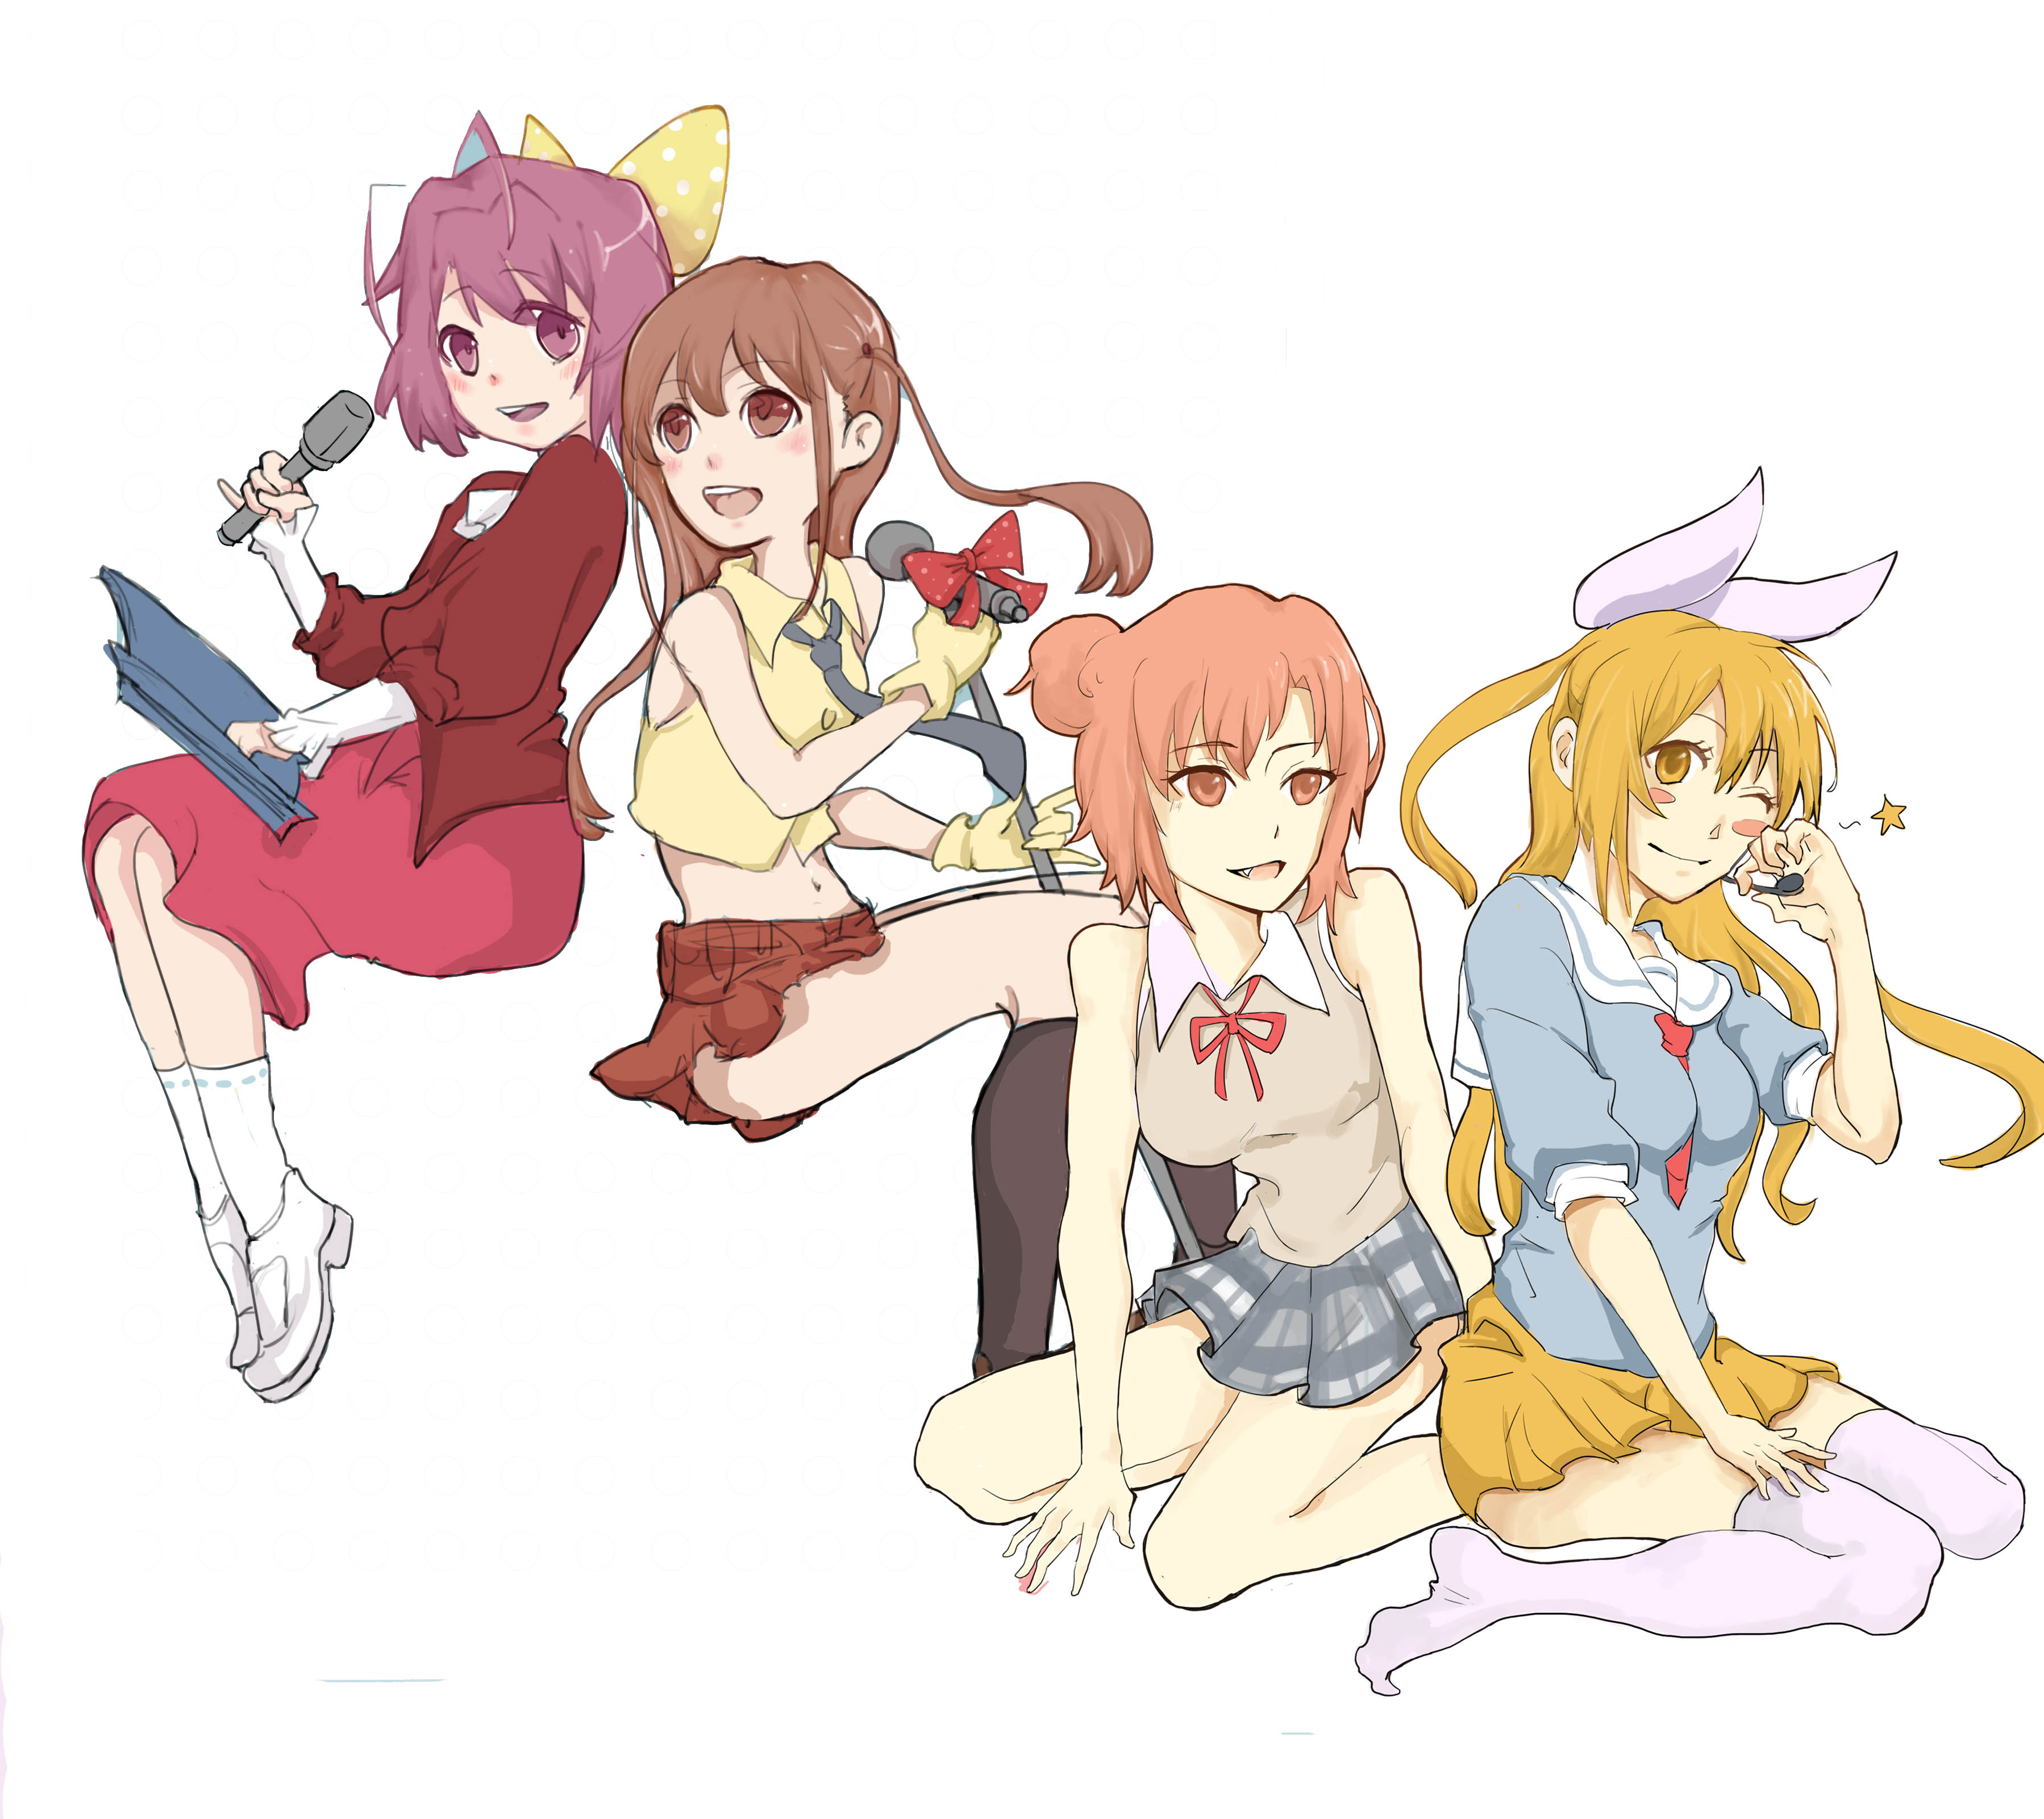
\includegraphics[width=11cm]{images/best4.jpg}}
\tiny\kai 图 by 阿七
\end{center}

\newpage
\section{03/12(日) 表演赛III~历代萌王}

{\kai\begin{longtable}{rrl}
\multicolumn{3}{l}{参赛人数: 376人\quad 合计投出: 1684票} \\
\multicolumn{3}{l}{\bfseries 日萌正统 } \\
1位 & 178票 & 雷姆@Re:从零开始的异世界生活 \\
2位 & 114票 & 木之本樱@魔卡少女樱 \\
3位 & 111票 & 鹿目圆香@魔法少女小圆 \\
4位 & 79票 & 逢坂大河@龙与虎 \\
5位 & 79票 & Saber@Fate/stay night \\
6位 & 69票 & 中野梓@轻音少女! \\
7位 & 43票 & 柊镜@幸运星 \\
8位 & 43票 & 园城寺怜@天才麻将少女阿知贺篇 \\
9位 & 40票 & 古手梨花@寒蝉鸣泣之时 \\
10位 & 39票 & 高町奈叶@魔法少女奈叶 \\
11位 & 31票 & 宫永咲@天才麻将少女 \\
12位 & 28票 & 巴麻美@魔法少女小圆 \\
13位 & 24票 & 翠星石@蔷薇少女 \\
14位 & 20票 & 原村和@天才麻将少女 \\
15位 & 10票 & 原田梨红@天使怪盗 \\
16位 & 3票 & 罗兹玛丽·阿普罗菲鲁特@明日的娜嘉 \\
\multicolumn{3}{l}{\bfseries 世度旁支 } \\
1位 & 110票 & 立华奏(天使)@Angel Beats! \\
2位 & 98票 & 五更琉璃(黑猫)@我的妹妹不可能这么可爱 \\
3位 & 94票 & 秋山澪@轻音少女 \\
4位 & 87票 & 千反田爱瑠@冰菓 \\
5位 & 82票 & 御坂美琴@某科学的超电磁炮 \\
6位 & 61票 & 五河琴里@约会大作战 \\
7位 & 57票 & 晓美焰@魔法少女小圆 \\
8位 & 55票 & 夏娜@灼眼的夏娜 \\
9位 & 47票 & 灰原哀@名侦探柯南 \\
10位 & 38票 & 南小鸟@LoveLive! \\
11位 & 26票 & 桂雏菊@旋风管家 \\
12位 & 18票 & 菲特·泰斯塔罗沙@魔法少女奈叶 \\
\end{longtable}}
